\section{Testing Taylor radii using only integers}\label{sec:taylor}
Can one test analytic continuation using the values of a prime product at integer cutoffs, without supplying a complex zero, a contour, or an oracle for evaluating an $L$-function? The answer for the three families is yes. The following construction converts a possible pole of a logarithmic derivative into a failure of an integer inequality for Taylor coefficients. Even a sequence of widely separated \emph{real} expansion centers detects zeros of arbitrarily large imaginary part.

\subsection*{The integer assertion}
Use $B=B_F$ and $C=C(d,H)$ from Section~\ref{sec:sentence}, with $B(0)=0$. Define integers
\[
 a_n=B(n)-B(n-1),\qquad
 b_n=a_n-2\bigl(B(\lfloor n/2\rfloor)-B(\lfloor(n-1)/2\rfloor)\bigr)\quad(n\ge1).
\]
Thus the second term subtracts $2a_{n/2}$ at even indices and vanishes at odd ones. For $N\ge1$, $1\le n\le N$, and Taylor order $k\ge0$, put
\begin{align*}
 J(n,N)&=\sum_{i=1}^{N(n-1)}\left\lfloor\frac{N^2}{N+i}\right\rfloor,\\
 A(c,k,N)&=\sum_{n=1}^N b_n J(n,N)^k (N!/n)^c,\qquad
 D(c,k,N)=k!\,N^{2k}(N!)^c .
\end{align*}
Here $0^0=1$. The division $N!/n$ is exact. For $c\ge5$, $j\ge1$ write
\[
 Q=2j,\qquad P=(2c-1)j-1,\qquad
 r=P/Q=c-\tfrac12-\tfrac1{2j},\qquad U=1000c\,C Q^3.
\]
At the given indices the test is
\begin{equation}\label{eq:taylor-packet}
   N P^k |A(c,k,N)|\ \le\
   D(c,k,N)\left(N Q^k U+9(d+1)P^k\right).
\end{equation}
Inputs to the field or conductor are quantified exactly as for the original test. For each such input take any of these three closed universal assertions.
\begin{center}\small
\begin{tabular}{@{}ll@{}}\toprule
Choice of disks & Indices tested, with all $k\ge0$, $N\ge1$\\\midrule
All disks & Every $c\ge5$ and $j\ge1$\\
One disk per center & Every $c\ge5$, with $j=c$\\
Exponentially spaced centers & $c=4+2^i$, $j=c$, for every $i\ge0$\\\bottomrule
\end{tabular}
\end{center}
Each matrix uses bounded sums, products, powers, factorials, integer quotients and truncated differences. In particular the formula has no numerical Taylor-coefficient parameter. The common denominator $D$ ensures that two separately accumulated nonnegative sums suffice for the signed numerator $A$.

\begin{theorem}\label{thm:taylor}
For each of the three analytic families, each of the three choices in the table characterizes the corresponding Riemann hypothesis in the classical standard model. The comparisons themselves are closed $\Pi^0_1$ formulas in iPRA.
\end{theorem}
\subsection*{Why these sums see a zero}
Put $D_F(s)=\sum a_n n^{-s}$ and $H_F(s)=\sum b_n n^{-s}$. At a prime power $n=p^l$ the logarithm of the integer product increases by at most $d\log p$. Elsewhere it is constant. Hence $0\le a_n\le d\log_2 n+1$, and these two series converge absolutely for $\Re s>1$. Reindexing the even terms there yields
\[
 H_F(s)=(1-2^{1-s})D_F(s).
\]
Writing $E(x)=B(\lfloor x\rfloor)-\Psi_F(x)/\log 2$, we have $|E(x)|\le1$. Summation by parts gives
\[
 D_F(s)=\frac{J_F(s)}{\log 2}
        +s\int_1^\infty E(x)x^{-s-1}\,dx ,
\]
with $J_F$ as in \eqref{eq:mellin}. The integral defines a holomorphic function for $\Re s>0$ by local dominated convergence, also after differentiation. The remaining term has the meromorphic continuation given by \eqref{eq:mellin}. At a zero shared by several field factors their logarithmic residues add with the same sign. Throughout $1/2<\Re s<1$, $|2^{1-s}|>1$, so the multiplier leaves this pole in place. It cancels the pole of $J_F$ at $s=1$. This gives a meromorphic function with which to compare the Taylor series on every disk.

\subsection*{The error of a finite coefficient}
The coefficient of $(c-s)^k$ at $s=c$ is
\[
 u_{c,k}=\frac{1}{k!}\sum_{n\ge1}\frac{b_n(\log n)^k}{n^c}.
\]
Absolute convergence near $c$ justifies differentiation term by term. For all the stated parameters we have the uniform estimate
\begin{equation}\label{eq:taylor-error}
 \left|u_{c,k}-\frac{A(c,k,N)}{D(c,k,N)}\right|\le\frac{9(d+1)}{N}.
\end{equation}
To see this, the right rectangle sum on $[1,n]$ with mesh $1/N$ is $\sum_{i=1}^{N(n-1)}1/(N+i)$. Its distance below the integral of $1/x$ is at most $1/N$, the difference of the left and right sums. Flooring the scaled summands costs at most $N(n-1)/N^2$. Thus $0\le\log n-J(n,N)/N^2\le n/N$. For $k\ge1$ the derivative of $t^k/k!$ on this interval is at most $e^{\log n}=n$, since $t^{k-1}/(k-1)!\le e^t$. For $k=0$ the approximation is exact term by term. Now $|b_n|\le3(d+1)n$. The total error below the cutoff is bounded by
\[
 \frac{3(d+1)}{N}\sum_{n=1}^N n^{3-c}\le\frac{6(d+1)}{N}.
\]
For the tail, $(\log n)^k/k!\le n$ gives a bound of $3(d+1)\sum_{n>N} n^{2-c}\le 3(d+1)/N$, by comparison with the integral of $x^{-2}$. This proves \eqref{eq:taylor-error}. It accounts for the additive term in \eqref{eq:taylor-packet}, including orders or prefixes for which the signed numerator vanishes.

\subsection*{Proof of Theorem~\ref{thm:taylor}}
Assume first the primary prime test for the chosen polynomial. The prefix of the signed coefficients telescopes to $S(x)=B(m)-2B(\lfloor m/2\rfloor)$, $m=\lfloor x\rfloor$. For $m=2n$ with $n\ge100$ the primary test bounds its absolute value by $C\sqrt n L(2n)^2$. At $m=2n+1$ add at most $d\log_2(2n+1)+1$. For $1\le m<200$ the elementary estimate $B(m)\le dm\log_2 m$ follows by bounding each prime-power jump of $\Psi_F/\log 2$. Using $L(m)\le2(1+\log m)$ and $\sqrt{200}<15$, all three cases give
\[
               |S(x)|\le 100 C\sqrt{x}(1+\log x)^2\qquad(x\ge1).
\]
Consequently $H_F(s)=s\int_1^\infty S(x)x^{-s-1}\,dx$ extends holomorphically to $\Re s>1/2$. On the circle $|s-c|=r$, we have $|s|\le2c$ and $\Re s\ge1/2+1/Q$. Substitution $x=e^t$ evaluates the integral majorant as
\[
   \int_0^\infty(1+t)^2e^{-t/Q}\,dt=Q+2Q^2+2Q^3\le5Q^3.
\]
Thus $|H_F|\le U$ there. Cauchy's coefficient estimate gives $r^k|u_{c,k}|\le U$. Combining with \eqref{eq:taylor-error} and clearing the positive denominators gives \eqref{eq:taylor-packet}. The family-specific implication from the complex zero hypothesis to the primary test is Proposition~\ref{prop:forward}.

Conversely \eqref{eq:taylor-packet} for every $N$ bounds $r^k|A/D|$ by $U+9(d+1)r^k/N$. Let $N$ tend to infinity at fixed $c,j,k$ and use \eqref{eq:taylor-error}. The resulting bound $r^k|u_{c,k}|\le U$ for all $k$ implies absolute convergence on every smaller disk, by the geometric series. There the power series is holomorphic and agrees near its center with the meromorphic $H_F$. The identity theorem forces agreement throughout the disk and rules out every pole there.

Even the exponentially spaced centers suffice. Put $s=x+iy$ with $x>1/2$ and $a_c=1/2+1/(2c)$. The inequality $|s-c|<c-a_c$ is equivalent to
\[
              2c(x-a_c)>x^2+y^2-a_c^2 .
\]
Its left side is $2c(x-1/2)-1$, which increases without bound along $c=4+2^i$. The right side stays bounded for fixed $s$. Thus an off-line zero in the right half of the strip would lie in one of the disks where the Taylor test rules out its pole. The functional equation and the field and character identifications in Section~\ref{sec:families} finish the proof. In particular, restricting to the single center $c=5$ would lose the covering argument.

\paragraph{Finite failure and formal scope.}
On a chosen disk containing a genuine pole the Taylor coefficients cannot obey the displayed Cauchy bound at every order. For a violating order, increasing $N$ eventually separates the rational approximation from the allowance. This proves a classical finite-detection statement and gives a primitive-recursive test of a \emph{supplied} failure. Its analytic premise supplies no numerical a priori bound on the first failing disk or order. The file \code{TaylorPackets.lean} constructs all nine closed sentences and interprets the finite sums. The kernel checks the arithmetic interpretation. The identification of their limits and radii with the meromorphic function is the mathematical argument above.
\subsection*{A constructive analytic consequence with a precision bound}
The universal integer tests supply a way to evaluate a continuation. Choose a diagonal disk, a complex rational point $s$ in it, and an integer $v\ge2$ such that $|c-s|\le r(1-1/v)$. This margin can itself be checked by squaring rationals. Given precision $t$, take
\[
 L=v(t+1+vU),\qquad N=2^{t+1}\,9(d+1)(L+1)(1+c)^L .
\]
Return the complex rational $\sum_{k<L}(A(c,k,N)/D(c,k,N))(c-s)^k$. Under the Taylor test it approximates the series to absolute error $2^{-t}$. Indeed, set $q=1-1/v$. Bernoulli's inequality gives $(1+1/(v-1))^v\ge2$ and hence $q^v\le1/2$. The tail from $L$ is at most $vUq^L\le2^{-t-1}$. In the retained terms, \eqref{eq:taylor-error} gives total approximation error at most $9(d+1)L(1+c)^L/N\le2^{-t-1}$. Every loop bound and rational required for this evaluation is primitive recursive in the displayed data. This is a conditional modulus and describes a particularly expensive algorithm.

There is also a direct compatibility check on overlapping diagonal disks. If $c'>c$, expand the exponential in the defining series for $u_{c,k}$ to get
\[
  u_{c,k}=\sum_{m\ge0}\binom{k+m}{k}(c'-c)^m u_{c',k+m}.
\]
The absolute double sum is bounded by $\sum |b_n|n^{-c}(\log n)^k/k!$: summing over $m$ contributes $\exp((c'-c)\log n)=n^{c'-c}$. This converges by the same estimate as in \eqref{eq:taylor-error}. Further, $c'-c+r_c<r_{c'}$ for diagonal radii $r_c=c-1/2-1/(2c)$. Thus on a smaller closed subdisk the translated power series may be expanded and regrouped absolutely by the binomial theorem, giving exactly the coefficients displayed above. The prescribed local values therefore agree. This establishes the overlap identity by a coefficient calculation. An internal derivation covering the entire construction of Cauchy names from prime-product data remains open in this Lean development.

For example, the rational point $3/4+5i$ is outside the scheduled disk centered at $36$ and inside the one centered at $68$. The membership comparison is a strict comparison of squared rational distances. The point illustrates the covering and carries no claim about a zero.

\begin{center}
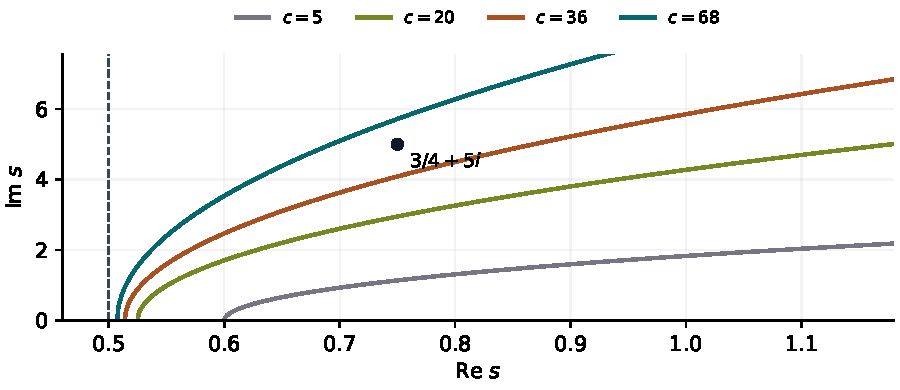
\includegraphics[width=.84\linewidth]{figures/disk_cover.pdf}\\[-1pt]
{\small Upper boundaries of four scheduled disks near the critical line. For each center, the portion below its curve and to the right of its left endpoint is inside the disk.}
\end{center}
